\documentclass[11pt,a4paper]{article}

\usepackage[margin=1in]{geometry}
\usepackage{amsmath,amssymb}
\usepackage{graphicx}
\usepackage{booktabs}
\usepackage{array}
\usepackage{multirow}
\usepackage{siunitx}
\usepackage{caption}
\usepackage{subcaption}
\usepackage{hyperref}
\usepackage{xcolor}

\graphicspath{{figures/}{./}}

\sisetup{
  round-mode=places,
  round-precision=4,
  table-number-alignment=center
}

\title{Exercise 3.1: Learning-Based Signal Detection for OFDM Systems}
\author{}
\date{}

\begin{document}

\maketitle

\section{Problem Background}

Exercise 3.1 studies learning-based signal detection for OFDM systems based on the deep learning receiver introduced in Section 3.1 and reference~\cite{ye2017power}. The reference method treats the OFDM transmitter, wireless channel, and receiver front-end as a black-box system. Instead of explicitly estimating the channel state information (CSI) and then performing symbol detection, the fully connected deep neural network (FC-DNN) directly maps the received OFDM samples to the transmitted bit vector.

The reference system uses an OFDM configuration with 64 subcarriers. The DNN input is formed from one received pilot OFDM block and one received data OFDM block. Since each OFDM block contains 64 complex subcarrier values, and each complex value is represented by its real and imaginary parts, the input dimension is
\begin{equation}
    2 \times 64 \times 2 = 256 .
\end{equation}
In the original QPSK setting, each OFDM data symbol carries
\begin{equation}
    64 \times \log_2 4 = 128
\end{equation}
transmitted bits. The reference design divides these 128 bits into eight groups, and each FC-DNN predicts one group of 16 bits. Therefore, the original per-group FC-DNN architecture is
\begin{equation}
    256 \rightarrow 500 \rightarrow 250 \rightarrow 120 \rightarrow 16 .
\end{equation}

\section{Task (a): FC-DNN Input and Output Dimensions for 64-QAM}

In this task, the OFDM system has 64 subcarriers and uses 64-QAM modulation. The problem assumes that eight identical FC-DNNs are used to recover the transmitted bits.

\subsection{Input Layer Size}

The input consists of the received pilot OFDM block and the received data OFDM block. Each block contains 64 complex subcarrier values. After separating real and imaginary parts, each block contributes 128 real-valued features. Therefore, the input dimension is
\begin{equation}
    N_{\mathrm{in}}
    = 2 \times 64 \times 2
    = 256 .
\end{equation}
The input layer size is therefore
\begin{equation}
    \boxed{256}.
\end{equation}

\subsection{Output Layer Size}

For 64-QAM, each modulated symbol carries
\begin{equation}
    \log_2 64 = 6
\end{equation}
bits. Since the OFDM symbol contains 64 subcarriers, the total number of transmitted bits in one OFDM data symbol is
\begin{equation}
    64 \times 6 = 384 .
\end{equation}
If eight identical FC-DNNs are used, each DNN predicts
\begin{equation}
    \frac{384}{8} = 48
\end{equation}
bits. Thus, the output layer size of each FC-DNN is
\begin{equation}
    \boxed{48}.
\end{equation}

Therefore, the per-DNN architecture for the 64-QAM setting becomes
\begin{equation}
    \boxed{
    256 \rightarrow 500 \rightarrow 250 \rightarrow 120 \rightarrow 48
    } .
\end{equation}

\subsection{Whether One DNN is Sufficient for BER Evaluation}

Simulating only one FC-DNN is not sufficient for a complete BER evaluation. One DNN only predicts one slice of the transmitted bit vector. In the 64-QAM case, one DNN predicts 48 bits out of the full 384-bit data symbol. The final BER should be computed over all predicted transmitted bits, so the outputs of all eight DNNs should be concatenated before calculating BER.

A single DNN may be used only as a rough sanity check if all eight bit groups are assumed to have identical statistical behavior. However, this does not provide a full BER evaluation because different bit groups may correspond to different subcarrier positions or bit positions within the modulation symbols. Therefore, the complete evaluation should use all eight FC-DNNs.

\section{Simulation Setup}

The implemented simulation follows the same high-level OFDM detection task as reference~\cite{ye2017power}. The main settings are summarized in Table~\ref{tab:setup}.

\begin{table}[h]
\centering
\caption{Main simulation settings.}
\label{tab:setup}
\begin{tabular}{ll}
\toprule
Item & Setting \\
\midrule
Number of subcarriers & 64 \\
Input feature dimension & 256 \\
Pilot settings & 8 pilots and 64 pilots \\
SNR values & 5, 10, 15, 20, 25 dB \\
Task (b) modulation & QPSK \\
Task (c) modulation & 64-QAM \\
Task (d) modulation & QPSK \\
Traditional baselines & LS and LMMSE/MMSE-type detector \\
Neural detector & FC-DNN \\
Metric & Bit error rate (BER) \\
\bottomrule
\end{tabular}
\end{table}

The DNN detector uses received pilot and data observations as inputs and predicts the transmitted bit vector. For the eight-DNN design, the transmitted bit vector is divided into eight groups. For the single-DNN design in Task~(d), one DNN directly predicts all transmitted bits.

\section{Task (b): QPSK BER Reproduction}

Task~(b) asks us to reproduce the BER curves corresponding to Fig.~3.3 in the exercise statement. The reproduced curves compare the FC-DNN detector with LS and LMMSE/MMSE-type baselines under QPSK modulation.

\begin{figure}[h]
\centering
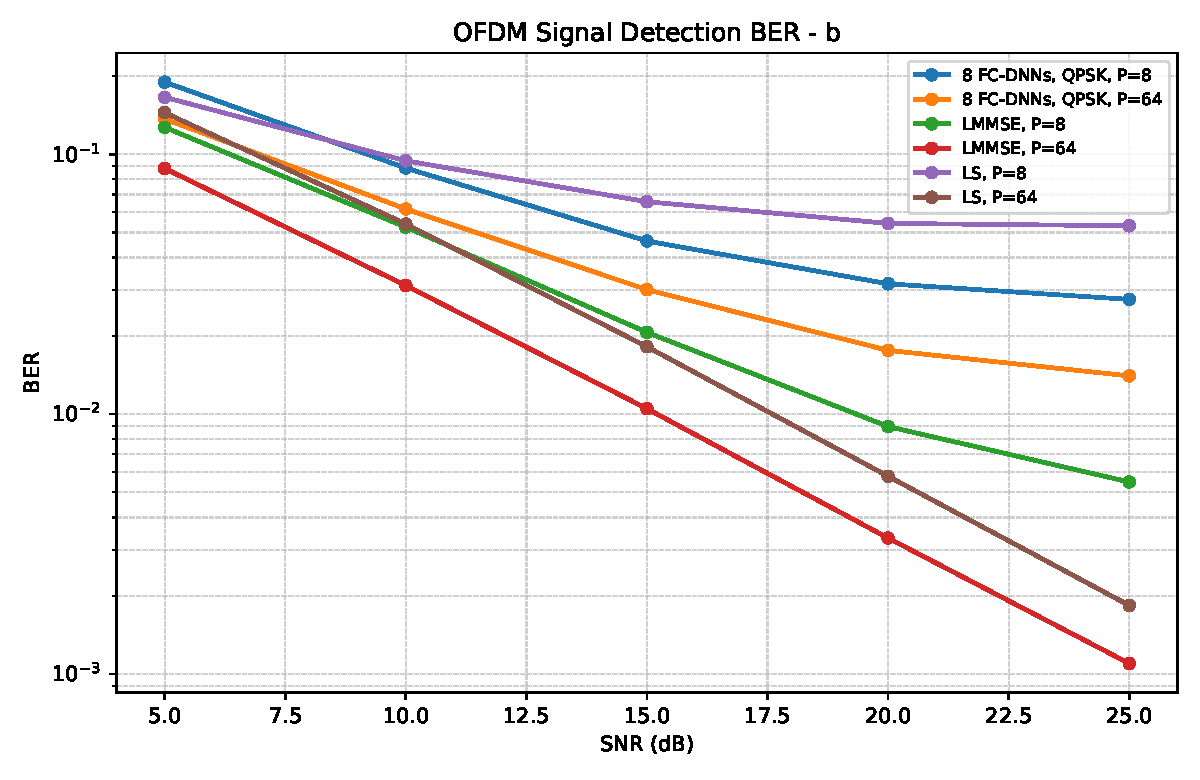
\includegraphics[width=0.82\linewidth]{ber_b.pdf}
\caption{Task (b) QPSK BER comparison among FC-DNN, LS, and LMMSE with 8 and 64 pilots.}
\label{fig:ber_b}
\end{figure}

\begin{table}[h]
\centering
\caption{Task (b) QPSK BER results.}
\label{tab:ber_b}
\resizebox{\linewidth}{!}{
\begin{tabular}{llccccc}
\toprule
Method & Pilots & 5 dB & 10 dB & 15 dB & 20 dB & 25 dB \\
\midrule
LS & 64 & 0.1445 & 0.0539 & 0.0182 & 0.0058 & 0.0018 \\
LS & 8  & 0.1656 & 0.0943 & 0.0656 & 0.0542 & 0.0530 \\
LMMSE & 64 & 0.0881 & 0.0313 & 0.0105 & 0.0033 & 0.0011 \\
LMMSE & 8  & 0.1269 & 0.0524 & 0.0206 & 0.0090 & 0.0055 \\
8 FC-DNNs & 64 & 0.1367 & 0.0615 & 0.0301 & 0.0176 & 0.0140 \\
8 FC-DNNs & 8  & 0.1894 & 0.0884 & 0.0463 & 0.0317 & 0.0276 \\
\bottomrule
\end{tabular}
}
\end{table}

The reproduced results show the expected qualitative behavior that BER decreases as SNR increases. The 64-pilot setting also performs better than the 8-pilot setting for all methods. This is consistent with the intuition that more pilots provide better information for channel estimation or implicit channel inference.

However, the reproduction is only partial. In the reference result, the deep learning detector is reported to be comparable to MMSE when enough pilots are used and more robust than conventional methods when fewer pilots are used. In the current implementation, the FC-DNN learns meaningful SNR-dependent detection behavior, but LMMSE remains stronger than FC-DNN, especially at high SNR. For example, at 25 dB with 64 pilots, the FC-DNN BER is 0.0140, whereas the LMMSE BER is 0.0011. With 8 pilots at 25 dB, the FC-DNN BER is 0.0276, whereas the LMMSE BER is 0.0055.

Therefore, the current result should be interpreted as an independent reproduction attempt that captures the main BER trend, but does not fully match the performance claim of the reference Fig.~3.3.

\section{Task (c): 64-QAM BER Results}

Task~(c) changes the modulation scheme from QPSK to 64-QAM while keeping the other settings unchanged. Since 64-QAM carries six bits per symbol, each OFDM data symbol contains 384 transmitted bits. With eight FC-DNNs, each DNN predicts 48 bits.

\begin{figure}[h]
\centering
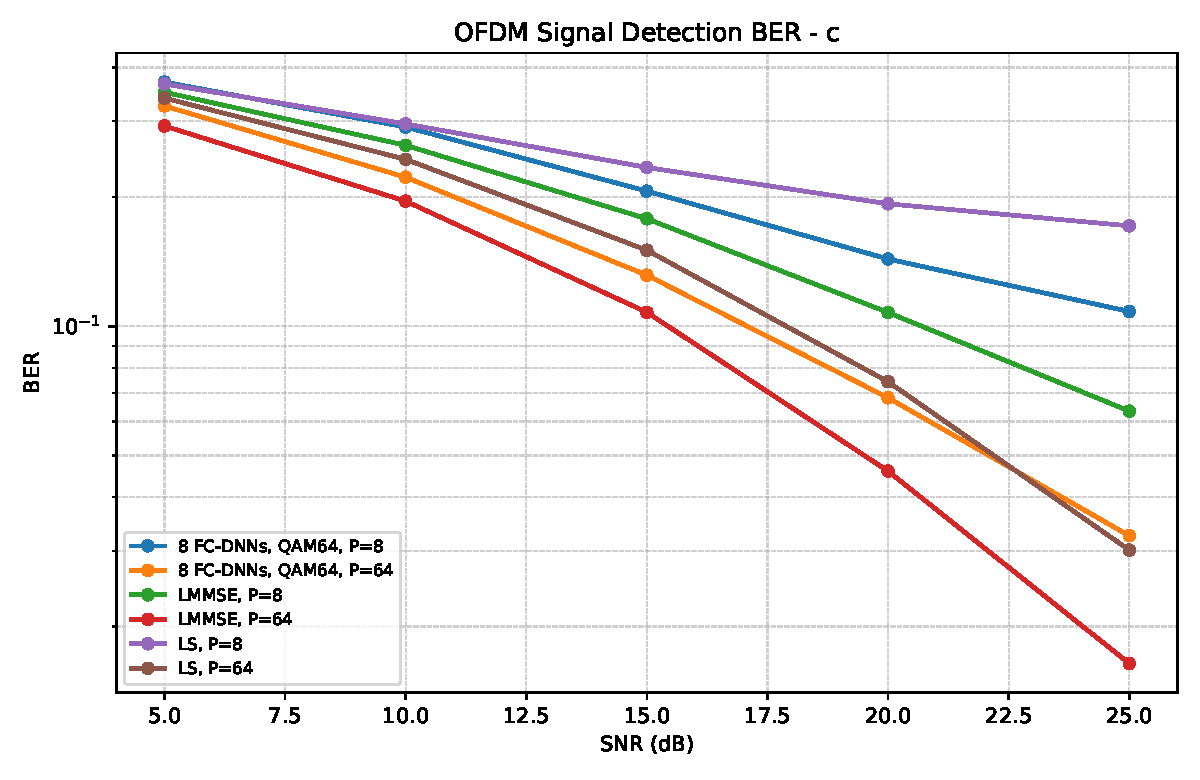
\includegraphics[width=0.82\linewidth]{ber_c.pdf}
\caption{Task (c) 64-QAM BER comparison among FC-DNN, LS, and LMMSE with 8 and 64 pilots.}
\label{fig:ber_c}
\end{figure}

\begin{table}[h]
\centering
\caption{Task (c) 64-QAM BER results.}
\label{tab:ber_c}
\resizebox{\linewidth}{!}{
\begin{tabular}{llccccc}
\toprule
Method & Pilots & 5 dB & 10 dB & 15 dB & 20 dB & 25 dB \\
\midrule
LS & 64 & 0.3395 & 0.2445 & 0.1502 & 0.0743 & 0.0301 \\
LS & 8  & 0.3664 & 0.2957 & 0.2341 & 0.1927 & 0.1712 \\
LMMSE & 64 & 0.2924 & 0.1954 & 0.1077 & 0.0460 & 0.0164 \\
LMMSE & 8  & 0.3504 & 0.2636 & 0.1778 & 0.1076 & 0.0634 \\
8 FC-DNNs & 64 & 0.3255 & 0.2222 & 0.1314 & 0.0681 & 0.0325 \\
8 FC-DNNs & 8  & 0.3699 & 0.2907 & 0.2062 & 0.1433 & 0.1082 \\
\bottomrule
\end{tabular}
}
\end{table}

Compared with the QPSK results in Task~(b), the 64-QAM BER values are significantly higher. This is expected because 64-QAM has a denser constellation than QPSK. Under the same average symbol power, the Euclidean distance between neighboring constellation points is smaller. Therefore, 64-QAM is more sensitive to AWGN, channel estimation error, and residual detection error.

The results also show that the pilot number remains important. With 64 pilots, all methods perform better than with 8 pilots. The FC-DNN detector still learns a decreasing BER trend as SNR increases, but the BER remains higher than the LMMSE baseline in the current implementation.

Overall, Task~(c) confirms that changing from QPSK to 64-QAM increases the detection difficulty. The output layer dimension must also be changed from 16 to 48 for each of the eight FC-DNNs.

\section{Task (d): Single FC-DNN versus Eight FC-DNNs}

Task~(d) trains a single FC-DNN to predict all transmitted bits in the OFDM data symbol. For QPSK with 64 subcarriers, the full transmitted bit vector contains
\begin{equation}
    64 \times 2 = 128
\end{equation}
bits. Therefore, the single-DNN architecture is
\begin{equation}
    256 \rightarrow 500 \rightarrow 250 \rightarrow 120 \rightarrow 128 .
\end{equation}
This is compared with the eight-DNN design, where each DNN predicts 16 bits.

\begin{figure}[h]
\centering
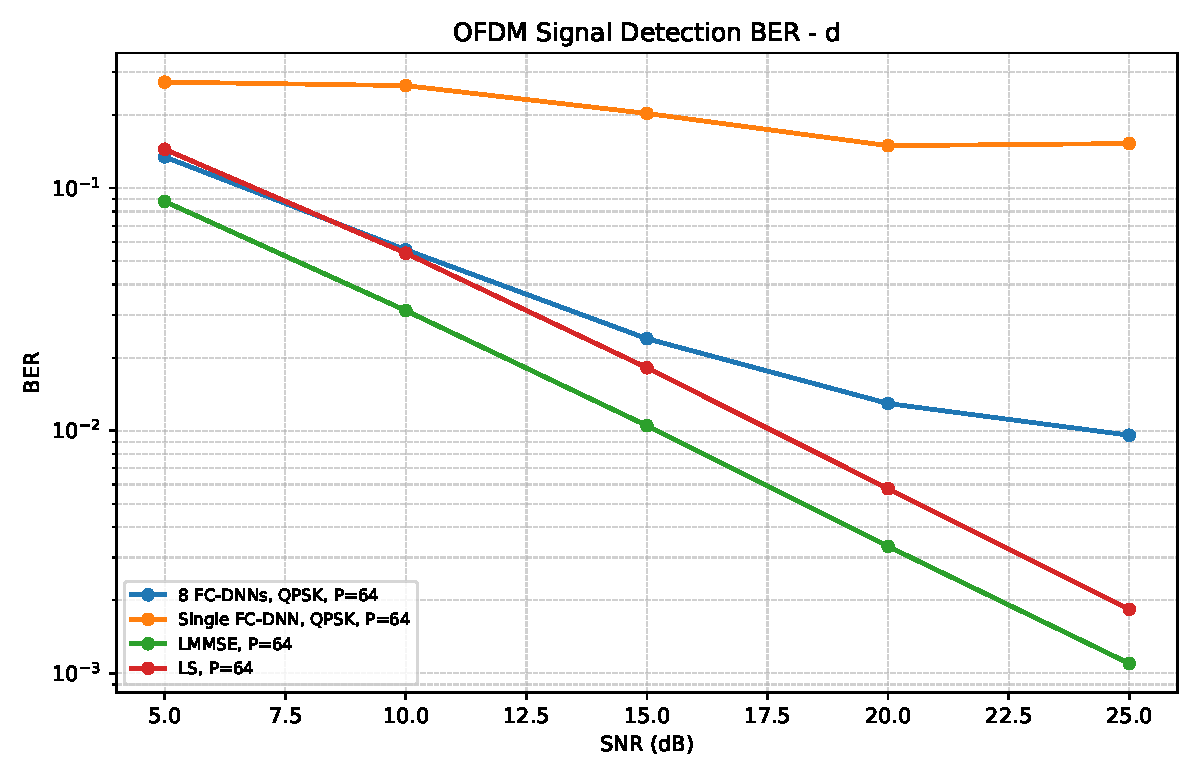
\includegraphics[width=0.82\linewidth]{ber_d.pdf}
\caption{Task (d) BER comparison between the eight-FC-DNN design and the single-FC-DNN design under QPSK with 64 pilots.}
\label{fig:ber_d}
\end{figure}

\begin{table}[h]
\centering
\caption{Task (d) QPSK BER comparison between single FC-DNN and eight FC-DNNs.}
\label{tab:ber_d}
\resizebox{\linewidth}{!}{
\begin{tabular}{lccccc}
\toprule
Method & 5 dB & 10 dB & 15 dB & 20 dB & 25 dB \\
\midrule
LS, 64 pilots & 0.1445 & 0.0539 & 0.0182 & 0.0058 & 0.0018 \\
LMMSE, 64 pilots & 0.0881 & 0.0313 & 0.0105 & 0.0033 & 0.0011 \\
8 FC-DNNs, 64 pilots & 0.1344 & 0.0556 & 0.0239 & 0.0129 & 0.0096 \\
Single FC-DNN, 64 pilots & 0.2734 & 0.2644 & 0.2030 & 0.1495 & 0.1526 \\
\bottomrule
\end{tabular}
}
\end{table}

The eight-FC-DNN design performs much better than the single-FC-DNN design in the current experiment. At 25 dB, the eight-FC-DNN detector reaches a BER of 0.0096, while the single-FC-DNN detector has a BER of 0.1526. The single-FC-DNN result also does not show a smooth monotonic decrease from 20 dB to 25 dB, suggesting that the model is harder to optimize.

This result indicates that directly predicting the full 128-bit vector with one FC-DNN is significantly more difficult than predicting smaller bit groups with eight separate FC-DNNs. A likely reason is that the single model must learn all bit positions jointly using one shared hidden representation. The optimization problem is more difficult, and the hidden layers may not provide enough capacity for the full-output prediction task.

However, this comparison is not fully parameter-matched. The eight-DNN design uses eight independent networks and therefore has more total parameters than the single-DNN design. Thus, the conclusion should be stated carefully: in the implemented setting, the eight-DNN design gives much better BER, but a larger or better-regularized single-DNN model might reduce the gap.

\section{Discussion}

The main findings are summarized as follows.

\begin{enumerate}
    \item For the 64-subcarrier OFDM system, the FC-DNN input dimension is 256 because the input consists of the real and imaginary parts of one received pilot block and one received data block.

    \item For 64-QAM, each OFDM data symbol contains 384 transmitted bits. If eight FC-DNNs are used, each DNN should output 48 bits.

    \item Simulating only one FC-DNN is not sufficient for full BER evaluation because the complete transmitted bit vector is split across all eight DNNs.

    \item In Task~(b), the QPSK experiment reproduces the expected qualitative trend that BER decreases with SNR and improves with more pilots. However, the current FC-DNN implementation does not fully reproduce the reference performance level, since LMMSE remains stronger.

    \item In Task~(c), 64-QAM gives worse BER than QPSK because the constellation points are closer together, making the detector more sensitive to noise and channel estimation error.

    \item In Task~(d), the eight-FC-DNN design performs much better than the single-FC-DNN design in the implemented setting. This suggests that predicting smaller bit groups is easier than predicting the entire transmitted bit vector with one network.
\end{enumerate}

\section{Reproducibility Note}

The maintained implementation entry point is
\begin{verbatim}
DNN_Detection/run_ofdm_detection.py
\end{verbatim}
The reproduced numerical results are stored in
\begin{verbatim}
outputs/ofdm_detection/results_b.csv
outputs/ofdm_detection/results_c.csv
outputs/ofdm_detection/results_d.csv
\end{verbatim}
and the corresponding BER figures are stored in
\begin{verbatim}
outputs/ofdm_detection/figures/ber_b.pdf
outputs/ofdm_detection/figures/ber_c.pdf
outputs/ofdm_detection/figures/ber_d.pdf
\end{verbatim}

The full local project also contains large channel datasets and model artifacts. These files may be omitted from lightweight review archives because the compressed project exceeds the upload limit. The project tree file records the complete local project structure.

\section{Conclusion}

Exercise 3.1 was completed by deriving the required FC-DNN input and output dimensions, reproducing QPSK BER curves, extending the simulation to 64-QAM, and comparing the original eight-DNN design with a single-DNN detector. The implemented FC-DNN detector learns meaningful BER behavior, but the reproduction of the reference deep learning performance is partial rather than exact. The final results support the main conceptual conclusions: input/output dimensions must be adjusted according to the modulation order, high-order modulation is harder to detect, and dividing the transmitted bit vector across several smaller FC-DNNs can be easier than predicting all bits with one single FC-DNN.

\begin{thebibliography}{9}

\bibitem{ye2017power}
H. Ye, G. Y. Li, and B.-H. F. Juang,
``Power of Deep Learning for Channel Estimation and Signal Detection in OFDM Systems,''
\emph{arXiv:1708.08514}, 2017.

\end{thebibliography}

\end{document}